\subsection[Forward-Backward algorithm]{Using the Model for
  Estimations: the Forward-Backward algorithm}
\label{sec:fb}

\begin{frame}
  \frametitle{$\alpha$ (forward) variables}
  \begin{itemize}
  \item Can we \emph{efficiently} compute $P(O \vert \lambda)$?\\
    \vspace*{.5em} Yes, using the \textbf{forward-backward} algorithm
    \vspace*{1em} \pause
  \item Introducing $\alpha$ (forward) variables:
    \begin{equation}
      \label{eq:alpha}
      \begin{split}
        \alpha_{t,i}=P(o_1,o_2,\ldots,o_t, q_t = S_i \vert \lambda) \\
        \scriptstyle{1 \le t \le T, 1 \le i \le N}
      \end{split}
    \end{equation}
    \pause
  \item Relation between $P(O \vert \lambda)$ and $\alpha$ variables:
    \begin{equation}
      \label{eq:eq1toalpha}
      P(O \vert \lambda) = \displaystyle\sum_{i=1}^{N}\alpha_{T,i}
    \end{equation}
  \end{itemize}
\end{frame}


\begin{frame}
  \frametitle{Computing $\alpha$ variables}
  \begin{columns}
    \column{0.38\textwidth}
    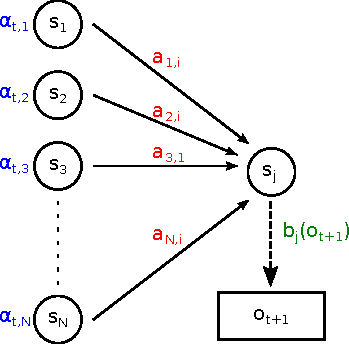
\includegraphics[width=\textwidth]{graphics/forward.pdf}
    \column{0.62\textwidth}
    \begin{itemize}
    \item $\alpha$ variables initialization \\
      $P(o_1,q_1=s_i) = P(o_1 \vert q_1=s_i)P(q_1=s_i)$ \\
      $\alpha_{1,i}=\pi_ib_i(o_1), \quad 1 \le i \le N$ \pause
    \item Induction step
      \begin{equation*}
        \label{eq:alpha_induct}
        \alpha_{t+1,j}=\Big[ \displaystyle\sum_{i=1}^{N}\alpha_{t,j}a_{i,j}\Big] b_{j}(o_{t+1}), \quad \substack{1 \le t \le T-1, \\ 1 \le j \le N}
      \end{equation*}
    \item Probability of the observed sequence
      \begin{equation*}
        \label{eq:alpha_term}
        P(O \vert \lambda) = \displaystyle\sum_{i=1}^{N}\alpha_{T,i}
      \end{equation*}
    \end{itemize}
  \end{columns}
\end{frame}

\begin{frame}
  \frametitle{$\beta$ (backward) variables}
  \begin{itemize}
  \item Introducing $\beta$ (backward) variables:
    \begin{equation}
      \label{eq:beta}
      \beta_{t,i}=P(o_{t+1} o_{t+2} \cdots o_{T} \vert q_t = S_i, \lambda)
    \end{equation}
    \vspace*{1em} \pause
  \item $\beta$ variables are not needed to compute $P(O \vert
    \lambda)$, but they are useful for the other two problems
  \item $\beta$ variables can be computed in a similar (efficient) way
    to the procedure for the $\alpha$ variables
  \end{itemize}
\end{frame}

\begin{frame}
  \frametitle{Computing $\beta$ variables}
  \begin{columns}[B]
    \column{0.55\textwidth}
    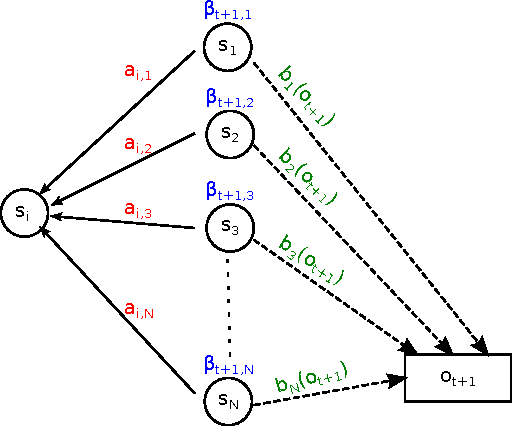
\includegraphics[width=\textwidth]{graphics/backward.pdf}
    \column{0.4\textwidth}
    \begin{itemize}
    \item $\beta$ variables initialization \\
      $\beta_{T,i}=1,\quad 1 \le i \le N$
    \end{itemize}
  \end{columns}
  \begin{itemize}
  \item Induction step \\
    $\beta_{t,i}=\displaystyle\sum_{j=1}^{N}a_{i,j}b_j(o_{t+1})\beta_{t+1,j},
    \quad t = T-1, T-2, \ldots , 1, 1 \le i \le N$
  \end{itemize}
\end{frame}

\begin{frame}
  \frametitle{Scaling problems}
  \begin{itemize}
  \item Remember $P(O \vert \lambda)$:
    \begin{equation*}
      P(O \vert \lambda) =  \displaystyle\sum_{\text{all}\;Q} \Big( \pi_{q_1} \cdot
      b_{q_1}(o_1) \cdot \displaystyle\prod_{t=2}^{T} b_{q_t}(o_t)
      a_{q_{t-1},q_t} \Big)
    \end{equation*}
    \pause
  \item for large sequences, terms are very close to zero and exceed
    precision range
  \item a scaling mechanism is needed
  \end{itemize}
\end{frame}

\begin{frame}
  \frametitle{The Forward-Backward algorithm with scaling}
  \begin{itemize}
  \item $\hat{\alpha}_{t,i}$ - scaled $\alpha$ variables
  \item $\hat{\beta}_{t,i}$ - scaled $\beta$ variables \vspace*{1em}
  \item $C_t$ - scaling coefficients \vspace*{1em}
  \item Scaled $\alpha$ variables
    \begin{equation}
      \label{eq:scaled-alpha}
      \bar{\alpha}_{t,i} = C_t \cdot \alpha_{t,i}
    \end{equation}
  \item Scaled $\beta$ variables
    
    \begin{equation}
      \label{eq:scaled-beta}
      \bar{\beta}_{t,j} = C_t \cdot \beta_{t,j}
    \end{equation}
  \end{itemize}
\end{frame}

\begin{frame}
  \frametitle{Computing scaled values}
  \begin{itemize}
  \item \emph{Scaled} intialization:
    \begin{align}
      \ddot{\alpha}_{1,i} = \alpha_{1,i},\quad 1 \le i \le N \\
      c_1 = \frac{1}{\displaystyle\sum_{i=1}^{N} \ddot{\alpha}_{1,i}} \\
      \hat{\alpha}_{1,i} = c_1 \cdot \ddot{\alpha}_{1,i}, \quad 1 \le
      i \le N
    \end{align}
    \pause
    \vspace*{-.5em}
  \item \emph{Scaled} induction step:
    \begin{align}
      \ddot{\alpha}_{t+1,i} = \Big[
      \displaystyle\sum_{i=1}^{N}\hat{\alpha}_{t,i}a_{i,j}\Big]
      b_{j}(o_{t+1}) \\
      c_{t+1} = \frac{1}{\displaystyle\sum_{i=1}^{N} \ddot{\alpha}_{t+1,i}} \\
      \hat{\alpha}_{t+1,i} = c_{t+1} \cdot \ddot{\alpha}_{t+1,i},
      \quad 1 \le i \le N
    \end{align}
  \end{itemize}

\end{frame}

\begin{frame}
  \frametitle{Computing $P(O | \lambda)$}
  \begin{equation}
    \label{eq:scaled-probability}
    P(O \vert \lambda) = \frac{1}{C_T}
  \end{equation}
\end{frame}


\begin{frame}
  \frametitle{Let's write some code}
  \begin{itemize}
  \item You will implement now the forward-backward algorithm in
    Octave
  \item Write code to compute:
    \begin{itemize}
    \item the
    \end{itemize}

  \end{itemize}
\end{frame}
